
Gracias a la criptografía de clave pública, podemos comunicarnos de forma 
segura y confidencial con 
las personas cuyas claves públicas tengamos, pero hay una serie de problemas 
que siguen sin resolverse. Por ejemplo, ¿cómo podemos comunicarnos con personas que 
nunca hemos conocido? ¿Cómo almacenamos las claves públicas y las revocamos? Más 
importante aún, ¿cómo lo hacemos a escala mundial, con millones de servidores y 
miles de millones de personas y dispositivos? Es una tarea difícil, pero para eso 
se creó la infraestructura de clave pública (PKI).

El objetivo de PKI es permitir una comunicación segura entre partes que nunca se 
han conocido antes. El modelo que usamos hoy se basa en “trusted third parties” 
llamados autoridades de certificación (\emph{CA}, a veces también llamadas autoridades 
de certificación) para emitir certificados en los que confiamos siempre. Una 
infraestructura PKI está formado por los siguientes agentes.


\subsubsection*{Suscriptor}


El suscriptor (o entidad final) es la parte que desea brindar servicios 
seguros, que requieren un certificado. Por ejemplo: una empresa que desea 
publicar su sitio web.

\subsubsection*{Autoridad de Registro}

La autoridad de registro (RA) lleva a cabo determinadas funciones de gestión 
relacionadas con la emisión de certificados. Por ejemplo, una RA puede realizar 
la validación de identidad necesaria antes de solicitar a una \emph{CA} que emita un 
certificado. En algunos casos, las RA también se denominan autoridades de 
registro local (LRA). En la práctica, muchas \emph{CA} también realizan tareas de RA.

\subsubsection*{Autoridad de certificación}

Una autoridad de certificación (\emph{CA}) es un agente en el que confiamos para emitir 
certificados que confirman las identidades de los suscriptores. También están 
obligados a proporcionar información de revocación actualizada en línea para 
que las partes que confían puedan verificar que los certificados siguen siendo válidos.

\subsubsection*{Consumidor de certificados}

Técnicamente, se trata de los navegadores web, de programas y de sistemas 
operativos que realizan la validación de certificados. Para ello, contienen 
almacenes que contienen los certificados de confianza de algunas \emph{CA}. En un 
sentido más amplio, los agentes que confían son los usuarios finales que 
dependen de certificados para una comunicación segura en Internet.

\subsubsection*{Certificados}

Un certificado es un documento digital que contiene una clave pública, cierta 
información sobre la entidad asociada y una firma digital del emisor del 
certificado. En otras palabras, es una herramienta que nos permite intercambiar, 
almacenar y usar claves públicas. Con eso, los certificados se convierten en 
el componente básico de PKI.

\subsubsection*{Cadenas de certificados}

En la mayoría de los casos, un certificado de una entidad final por sí solo es 
insuficiente para una validación exitosa. En la práctica, cada servidor debe 
proporcionar una cadena de certificados que conduzca a una raíz de confianza. 
Las cadenas de certificados se utilizan por motivos de seguridad, técnicos y 
administrativos.

\subsubsection*{Autoridades de certificación}

Las autoridades de certificación (\emph{CA}) son la parte más importante del modelo 
actual de confianza en Internet. Pueden emitir un certificado para cualquier 
nombre de dominio, lo que significa que todo lo que digan es válido. 
Durante mucho tiempo, el costo de los certificados era bastante elevado. 
Sin embargo, en estos días, el precio se redujo drásticamente, impulsado 
por una fuerte competencia, adicionando a varias organizaciones que proveen 
estos servicios de manera gratuita. 

\subsubsection*{Ciclo de vida del certificado}

El ciclo de vida del certificado comienza cuando un suscriptor prepara una 
Solicitud de firma de certificado (CSR) y la envía a la \emph{CA} de su elección. 
El propósito principal del CSR es poner a disposición de la \emph{CA} la clave 
pública, así como demostrar la propiedad de la clave privada correspondiente 
(mediante una firma). 


\begin{center}
    \begin{figure}   
       \begin{center}
          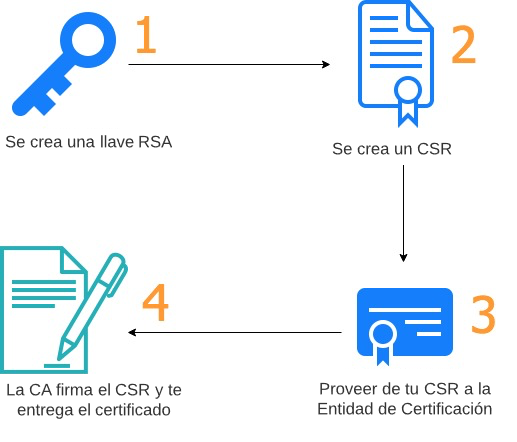
\includegraphics[width=9cm,height=8cm]{ca-process.png}
       \end{center}
       \caption{Solicitud de un certificado}
       \label{figSolCert}
    \end{figure}
 \end{center}

